\documentclass{article}

% \usepackage{listings}
\usepackage{graphicx}
\usepackage{xepersian}

\settextfont{Vazirmatn}

\begin{document}
\begin{titlepage}

    % Center everything on the page
    \centering

    % Title
    \vspace*{2cm}
    {\Huge \textbf{تمرین اول}} \\[1cm]
    
    % Subtitle
    {\LARGE درس مبانی برنامه نویسی و کامپیوتر} \\[2cm]
    
    % Author's name
    {\Large \textbf{دکتر ملکی مجد}} \\[0.5cm]
    
    % Date
    {\large \today} \\[4cm]
    
    % Semester
    {\large ترم پاییز ۴۰۳۱} \\[2cm]
    
    % Logo at the bottom
    
\includegraphics[width=0.2\textwidth]{iustlogo.png} \\[0.2cm]
    \textbf{دانشگاه علم و صنعت}
    
\end{titlepage}

\section{نکات}
\begin{enumerate}
    \item  پاﺳﺦ ﺗﻤﺎمی ﺳﻮاﻻت ﺗﻨﻬﺎ ﺑﺎ زﺑﺎن ﺳی ﻗﺎﺑﻞ ﻗﺒﻮل اﺳﺖ.
    \item در صورتی که در هر سؤال ابهام یا سوالی وجود داشت. حتما سعی کنید سؤال خود را
    در گروه درسی بپرسید تا دیگران نیز از پاسخ شما بهره‌مند شوند.
    \item در صورتی که از منابعی برای حل سوالات استفاده کرده اید حتما آن را به صورت کامنت
    در ابتدای کدخود بنویسید. همچنین اگر با دانشجو دیگری همفکری کرده اید حتما آن
    را نیز ذکر کنید.
    \item برای ارسال تمرین های خود در طول ترم مجموعا ۱۰ روز تاخیر مجاز وجود دارد. در
    صورتی که بیشتر از این مقدار تاخیر داشته باشید، نمره تمرین شما صفر خواهد شد.
    \item برای هر سری تمرین ۳ روز از ۱۰ روز تاخیر مجاز را می توانید استفاده کنید.
\end{enumerate}

\section{طراحان سؤال}
در صورتی که در هر سوالی ابهامی وجود دارد، میتونید از طریق آیدی های زیر سؤال خود را
مطرح کنید.

\begin{itemize}
    \item محمد یاوری - \lr{ID: @EmmWhy}

    \item بهاره کاوسی نژاد - \lr{ID: @Bahareh\_0281}
\end{itemize}

\pagebreak

\section{سوالات}

\subsection{برنامه ساده چاپ}
فرض کنید که شما عددی به نام \( N \) دریافت می‌کنید و هدف این است که یک شکل مثلثی متناسب با مقدار \( N \) چاپ کنید. این شکل به‌صورت زیر است:

\textbf{ورودی}: یک خط شامل \( n \) از 1 تا 100

\begin{itemize}
    \item اگر \( N = 1 \) باشد:
    \begin{verbatim}
        /\
    \end{verbatim}
    \item اگر \( N = 2 \) باشد:
    \begin{verbatim}
         /\
        \  /
    \end{verbatim}
    \item و اگر \( N = 3 \) باشد:
    \begin{verbatim}
          /\
         \  /
        \    /
    \end{verbatim}
\end{itemize}

\paragraph{توجه:} برای این که در تعداد اسپیس ها اشتباهی نکنید، پیشنهاد میشود که برنامه \lr{notepad} خود را باز کنید و از آنجا شکل مثلث را بنویسید و امتحان کنید. این برنامه، اسپیس ها همان اندازه ای را دارند که بقیه کاراکتر ها دارند.

\begin{figure}[h!]
    \begin{minipage}{0.4\textwidth}
        \centering
        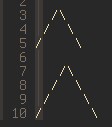
\includegraphics[width=0.5\textwidth]{q1-small.png}
    \end{minipage}
    \begin{minipage}{0.4\textwidth}
        \centering
        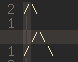
\includegraphics[width=0.5\textwidth]{q1-big.png}
    \end{minipage}
    \caption{استفاده از برنامه ای مشابه \lr{notepad} برای امتحان کردن شکل }
\end{figure}

\newpage

\section{چراغ قوه بازی!}
فرض کنید شما در حال طراحی یک بازی جستجوی گنج ساده برای افراد مبتدی هستید. در این بازی، بازیکن یک چراغ‌قوه دارد تا اتاق‌ها را بگردد. این چراغ‌قوه فقط وقتی بازیکن داخل اتاق است کار می‌کند و با خروج او خاموش می‌شود. با این حال، امتیاز کل بازیکن باید در طول بازی ذخیره شود و در هر بار ورود به اتاق‌ها به‌روز شود.

در این برنامه، ما از یک متغیر محلی برای نشان دادن وضعیت چراغ‌قوه استفاده می‌کنیم که تنها وقتی بازیکن در اتاق است، ایجاد و استفاده می‌شود. همچنین امتیاز کل در یک متغیر سراسری ذخیره می‌شود تا در تمام طول بازی وجود داشته باشد و با هر بار ورود به اتاق‌ها به‌روز شود.

یک برنامه‌ی ساده به زبان C بنویسید که دو نوع متغیر داشته باشد:

\begin{enumerate}
\item یک متغیر محلی به نام int flashlight که نشان‌دهنده وضعیت چراغ‌قوه است. این متغیر باید فقط وقتی بازیکن "داخل اتاق" است تعریف شود و با هر بار ورود بازیکن به اتاق دوباره مقداردهی شود.
\item یک متغیر سراسری به نام int totalScore که امتیاز کل بازیکن را در طول بازی نگه می‌دارد. این متغیر باید در بالای برنامه تعریف شود و هر بار که بازیکن وارد اتاق می‌شود، به‌روزرسانی شود.
\end{enumerate}
بازیکن تا وقتی که عدد منفی یک را دریافت نکرده، شماره اتاق را میگیرد و وارد اتاق میشود. اين شماره عددي بين 1 تا 9 است. اگر اين مقدار كوچكتر يا مساوي 5 بود به بازيكن 10 امتياز و اگر بين 6 تا 9 بود به بازيكن 20 امتياز اضافه مي شود.

 هر بار که بازیکن وارد یک اتاق می‌شود، مقدار totalScore را افزایش دهید و نشان دهید که چراغ‌قوه روشن است یا نه. در انتهاي بازي هنگامی که منفی یک را دریافت کردید نيز مقدار totalScore را چاپ كنيد.

توجه کنید که اگر بازیکن وارد اتاق جدیدی نشود و در اتاق قبلی باشد دیگر چراغ قوه اش خاموش روشن نمیشود! ولی امتیاز اتاق قبلی به امتیاز کل اضافه میشود.

\subsubsection{مثال ها:}
    \paragraph{توجه: } در بین علامت منفی و عدد ۱ فاصله‌ای وجود ندارد.
\begin{itemize}
    \item مثال ۱: 
    \begin{itemize}
        \item ورودی:
        \begin{LTR}
        \begin{verbatim}
            3
            7
            - 1
        \end{verbatim}
        \end{LTR}
        \item خروجی:
        \begin{LTR}
        \begin{verbatim}
            Flashlight is ON in room 3.
            Flashlight is OFF.
            Flashlight is ON in room 7.
            Flashlight is OFF.
            Total Score: 30
        \end{verbatim}
    \end{LTR}
    \end{itemize}
        \item مثال ۲:
        \begin{itemize}
            \item ورودی:
            \begin{LTR}
            \begin{verbatim}
                6
                4
                4
                - 1
            \end{verbatim}
            \end{LTR}
            \item خروجی:
            \begin{LTR}
            \begin{verbatim}
                Flashlight is ON in room 6.
                Flashlight is OFF.
                Flashlight is ON in room 4.
                Flashlight is OFF in room 4.
                Total Score: 40
            \end{verbatim}
            \end{LTR}
        \end{itemize}

        \item مثال ۳:
        \begin{itemize}
            \item ورودی:
            \begin{LTR}
            \begin{verbatim}
                2
                3
                9
                - 1
            \end{verbatim}
            \end{LTR}
            \item خروجی:
            \begin{LTR}
            \begin{verbatim}
                Flashlight is ON in room 2.
                Flashlight is OFF.
                Flashlight is ON in room 3.
                Flashlight is OFF.
                Flashlight is ON in room 9.
                Flashlight is OFF.
                Total Score: 40
            \end{verbatim}
            \end{LTR}
        \end{itemize}
\end{itemize}

\newpage

\subsection{شبه كد}
یک عدد دهدهی کوچک \( n \) (بین 0 تا 15) به برنامه داده می‌شود. برنامه باید معادل باینری چهار بیتی این عدد را به عنوان خروجی نمایش دهد.

\begin{itemize}
    \item \textbf{ورودی:} 5؛ \textbf{خروجی:} 0101
    \item \textbf{ورودی:} 10؛ \textbf{خروجی:} 1010
\end{itemize}

\textbf{سودوكد:}
\begin{LTR}
\begin{verbatim}
Start program

    bit4 = n % 2
    n = n / 2
    bit3 = n % 2
    n = n / 2
    bit2 = n % 2
    n = n / 2
    bit1 = n % 2

    Print bit1, bit2, bit3, bit4 as a 4-bit binary number

End program
\end{verbatim}
\end{LTR}

\newpage

\subsection{رمز خیلی امن}
فرض کنید شما مسئول امنیت یک بانک دیجیتالی هستید و نیاز دارید برنامه‌ای بنویسید که وقتی یک مشتری قصد ورود به سیستم را دارد، ویژگی‌های رمز عبور ورودی او را به دقت بررسی کند. برنامه باید در نهایت به کاربر اطلاع دهد که آیا رمز عبور او ایمن و مناسب است یا خیر.

\paragraph{قوانین امنیتی برنامه}
رمز عبور که یک عدد صحیح است باید شرایط زیر را داشته باشد:
\begin{itemize}
    \item بزرگ‌تر یا مساوی ۱۰ باشد. (اگر کمتر از 10 باشد ایمن نیست)
    \item اگر رمز عبور بزرگ‌تر از ۱۰ است و عددی زوج است، ایمن است.
    \item اگر رمز عبور بزرگ‌تر از ۱۰ باشد و عددی فرد باشد، ایمن نیست.
\end{itemize}

\paragraph{مراحل برنامه}
\begin{itemize}
    \item از کاربر یک رمز عبور (عدد) دریافت کنید.
    \item با استفاده از ساختار \lr{if-elif-else} قوانین امنیتی بالا را بررسی کنید.
    \item نتیجه مناسب را به کاربر نمایش دهید.
\end{itemize}

\paragraph{مثال‌های ورودی و خروجی:}
\begin{itemize}
    \item مثال ۱:
    \begin{itemize}
        \item ورودی: 12
        \item خروجی: \lr{Your password is secure.}
    \end{itemize}
    \item مثال ۲:
    \begin{itemize}
        \item ورودی: 4
        \item خروجی: \lr{Your password is not secure.}
    \end{itemize}
    \item مثال ۳:
    \begin{itemize}
        \item ورودی: 17
        \item خروجی: \lr{Your password is not secure.}
    \end{itemize}
\end{itemize}

\newpage

\subsection{مومو}

سارا مشغول کار کردن با گوشی‌اش بود که دید شخص ناشناسی در واتس‌اپ به او پیام داده است.

او که از ماجرای مومو خبر نداشت، پیام را جواب داد تا پی ببرد که این شخص ناشناس با این قیافه عجیب چه کسی است و با او چه کار دارد!

فردا اما توسط پیام‌هایی که توسط پلیس فتا که حواسش به همه جا هست پخش شده بود، متوجه شد که این شخص ناشناس مومو است و قصد هک کردن و در نهایت کشتن او را دارد!

سارا اما تصمیم به مقابله با مومو گرفت و به او گفت که او دانشجوی مهندسی کامپیوتر دانشگاه علم و صنعت است. مومو با دیدن این پیام وحشت کرد و متوجه شد که اگر سارا راست بگوید و سارا اطلاعات او را در دانشگاه پخش کند، ممکن است این بار خود او توسط دانشجویان و دوستان سارا هک شود.

بنابراین به سارا گفت که اگر راست می‌گویی، برای مطمئن شدن باید این سوال را بدون استفاده از حلقه‌ها و همچنین بدون استفاده از عملگرهای شرطی حل کنی. با توجه به تازه‌کار بودن سارا به او در حل این سوال کمک کنید.

در این سوال به شما خطی از اعداد داده می‌شود اما در بین این اعداد دو کاراکتر وجود دارد که باید آنها را تشخیص دهید.

\textbf{نکته:}
\begin{itemize}
    \item تضمین می‌شود که این دو کاراکتر در اول یا آخر خط نیامده‌اند.
    \item تضمین می‌شود که این دو کاراکتر پشت سر هم نیامده‌اند.
    \item در صورت استفاده از حلقه‌ها و عملگرهای شرطی نمره سوال را دریافت نخواهید کرد، اگر چه نمره شما در \lr{Quera} ۱۰۰ باشد.
\end{itemize}

\textbf{ورودی نمونه ۱:}
\begin{LTR}
\begin{verbatim}
111222233333T8887777666C5555444
\end{verbatim}
\end{LTR}

\textbf{خروجی نمونه ۱:}
\begin{LTR}
\begin{verbatim}
T C
\end{verbatim}
\end{LTR}


\end{document}